% Plantilla LLNCS para Springer Computer Science Proceedings
\documentclass[runningheads]{llncs}

\usepackage[T1]{fontenc}
\usepackage[utf8]{inputenc}
\usepackage{graphicx}
\usepackage{hyperref}
\usepackage{color}
\renewcommand\UrlFont{\color{blue}\rmfamily}

\begin{document}

\title{Búsqueda semántica de abstracts científicos mediante
indexación HNSW en bases de datos vectoriales}

\author{Santiago Callocondo-Garay\inst{1}\orcidID{0009-0007-2794-5097} \and
Piero Mejia-Ramos\inst{1}\orcidID{0009-0006-3011-0640}}

\authorrunning{S. Callocondo and P. Mejia}

\institute{Escuela Profesional de Ingeniería de Sistemas, Universidad Nacional de
San Agustín, Arequipa, Perú\\
\email{\{scallocondo,pmejia\}@unsa.edu.pe}}

\maketitle

\begin{abstract}
----

\keywords{HNSW, búsqueda semántica, embeddings científicos, FAISS, Recall@K}
\end{abstract}

% -------------------------------------------------------
\section{Introducción}
% -------------------------------------------------------

% Párrafo 1 — Marco conceptual: el problema general y su importancia
¿Cuánta literatura científica cabe hoy en un solo repositorio? A mayo de 2026,
ArXiv supera los 2,6 millones de artículos \cite{ref1} y PubMed indexa más de 38
millones de registros biomédicos \cite{ref2}. Ese volumen rompe la búsqueda por
palabras clave: dos abstracts pueden describir la misma idea sin compartir un solo
término. Para sortear ese obstáculo, los sistemas modernos representan cada
documento como un vector denso de alta dimensionalidad ---un \textit{embedding}---
capaz de capturar parecido semántico más allá del vocabulario literal \cite{ref3}.
La dificultad reaparece al consultar. Recuperar el vecino más cercano de forma
exacta obliga a comparar la consulta contra todos los vectores del corpus, un costo
$O(N \cdot d)$ que crece de forma lineal con el tamaño de la colección; sobre
millones de documentos, la latencia por consulta se dispara hasta volverse
impracticable para cualquier uso interactivo. Por eso la recuperación a gran escala
descansa en métodos de búsqueda aproximada del vecino más cercano (ANN), que ceden
una fracción mínima de exactitud a cambio de respuestas órdenes de magnitud más
veloces \cite{ref4}.

% Párrafo 2 — Antecedentes: lo que sabemos (HNSW como solución establecida)
Entre los algoritmos ANN, Hierarchical Navigable Small World (HNSW) \cite{ref5} se
ha consolidado como el estándar de facto para búsqueda semántica a gran escala.
Inspirado en la teoría de redes de mundo pequeño \cite{ref6}, organiza los vectores
en una jerarquía multi-capa donde las capas superiores permiten una navegación
global eficiente y la capa base concentra la conectividad local; el resultado es
una complejidad de consulta $O(\log N)$ con recalls superiores al 97\% en
benchmarks canónicos \cite{ref5}. Esta eficiencia ha motivado su adopción como
índice primario en plataformas de producción como FAISS \cite{ref7} y Milvus
\cite{ref8}. No obstante, el rendimiento del índice depende de dos factores
críticos: su parametrización interna y la métrica de similitud empleada.

% Párrafo 3 — Antecedentes específicos: los dos factores que determinan el rendimiento
La parametrización y la métrica de similitud determinan directamente la calidad y
velocidad de la recuperación. En cuanto a la parametrización, Zhao et al.~\cite{ref9}
demuestran que una poda jerárquica mediante el parámetro $\lambda$ reduce el tiempo
de construcción hasta $1.27\times$ manteniendo Recall@10 $>$ 97\% sobre SIFT1M,
lo que evidencia que los hiperparámetros $M$ y \textit{ef\_construction} gobiernan
el equilibrio entre velocidad de indexación y exactitud de recuperación. En cuanto
a la métrica, dentro de los sistemas de generación aumentada por recuperación
(RAG) \cite{ref10}, Elkiran y Rasheed \cite{ref11} evalúan coseno, producto interno
y L2 sobre el corpus SQuAD \cite{ref12}: coseno y producto interno alcanzan R@10
entre 0.909 y 0.925, mientras que L2 sobre vectores no normalizados colapsa
a R@10 $= 0.373$. Estos hallazgos, sin embargo, provienen de colecciones de
propósito general que no capturan las particularidades del lenguaje científico
especializado.

% Párrafo 4 — Vacío de conocimiento: lo que no sabemos
Ningún trabajo ha evaluado HNSW en corpus de abstracts científicos con vocabulario
especializado y distribución temática heterogénea. Los benchmarks disponibles se
limitan a imágenes o texto conversacional \cite{ref11,ref12}, sin considerar la
densidad terminológica ni la polisemia disciplinar propia de la literatura
académica. Tampoco existe un benchmark sistemático que combine modelos de embedding
científico ---como SciBERT o E5-large--- con un análisis controlado del impacto de
$M$ y \textit{ef\_construction} sobre métricas de recuperación (Recall@K, MRR) en
ese dominio. Esta ausencia limita la transferibilidad de las recomendaciones de
parametrización existentes a contextos reales de recuperación en literatura
científica.

% Párrafo 5 — Objetivo (estación terminal): exclusivamente el objetivo del trabajo
El presente trabajo evalúa experimentalmente HNSW indexado sobre FAISS para
búsqueda semántica de abstracts del dataset \textit{arxiv-abstracts-2021},
comparando los modelos SciBERT y E5-large bajo distintas configuraciones de $M$,
\textit{ef\_construction} y métrica de similitud, con el propósito de identificar
la parametrización óptima que maximice Recall@K y MRR minimizando la latencia de
consulta en corpus de literatura científica.

% -------------------------------------------------------
\section{Trabajos Relacionados}
% -------------------------------------------------------

Los algoritmos ANN surgen como solución práctica a la inviabilidad computacional de
k-NN exacto en espacios de alta dimensionalidad. Mathur y Chhabra \cite{ref4} los
clasifican en cuatro familias ---fuerza bruta, árboles, cuantización y grafos---,
y señalan a los métodos basados en grafos como los más competitivos cuando crece la
dimensión. HNSW \cite{ref5} encarna esa familia: levanta una jerarquía multi-capa
inspirada en las redes de mundo pequeño \cite{ref6}, donde las capas altas ofrecen
saltos largos y dispersos y la capa base afina la búsqueda local, con un costo de
consulta $O(\log N)$. Sobre esta idea base han surgido numerosas optimizaciones.
Iwasaki y Miyazaki \cite{ref13} ajustan los grados de entrada y salida de cada
nodo ---recortando aristas salientes redundantes sin perder exactitud--- para
acelerar las consultas en datos de alta dimensión. Xi Zhao et al.~\cite{ref14},
por su parte, atacan el costo de armado con LSH-APG, un esquema que apoya la
inserción de puntos en una búsqueda ligera basada en hashing sensible a la
localidad y permite mantener el grafo de forma incremental conforme el conjunto
crece.

El verdadero talón de Aquiles de HNSW no está en consultar, sino en construir. Cada
inserción dispara múltiples recorridos multi-capa y un aluvión de cálculos de
distancia \cite{ref9}. Feifan Zhao et al.~\cite{ref9} responden con H-DMax, que
introduce un parámetro $\lambda$ para podar vecinos lejanos de forma jerárquica
---severa en las capas bajas, prudente en las altas para no romper la conectividad
global---, y logran acelerar la construcción hasta $1.27\times$ perdiendo menos del
0.27\% de Recall@10 sobre SIFT1M ($\lambda=1.10$). La cuantización por producto
\cite{ref15} sigue otra ruta: comprime los vectores en códigos cortos y, dentro de
FAISS \cite{ref7}, ofrece la mayor aceleración de armado ($3.6\times$). El precio,
eso sí, es alto: el recall puede desplomarse hasta el 85\%, lo que la descarta
cuando la fidelidad no es negociable.

En el plano de la infraestructura, FAISS \cite{ref7} y Milvus \cite{ref8} marcan la
referencia para desplegar índices HNSW en producción. Milvus admite coseno,
producto interno y L2 sobre embeddings densos e híbridos, y es la base de muchos
pipelines RAG \cite{ref10} recientes. Sobre esa plataforma, Elkiran y Rasheed
\cite{ref11} ponen a prueba las tres métricas con embeddings de OpenAI
(3072 dimensiones) y el corpus SQuAD \cite{ref12}: coseno y producto interno rozan
R@10 $= 0.909$--$0.925$ y MRR $= 0.781$--$0.793$, frente al desplome de L2 sin
normalizar (R@10 $= 0.373$, MRR $= 0.116$). El umbral de similitud, como recuerda
la teoría clásica de recuperación de información \cite{ref16}, inclina la balanza
entre precisión y recall, y la normalización resulta decisiva cuando se trabaja
con L2.

La literatura revisada deja un hueco difícil de ignorar. Nadie ha medido HNSW sobre
abstracts científicos, con su vocabulario denso y su reparto temático desigual.
Tampoco existe un banco de pruebas que enfrente modelos de embedding científico
como SciBERT o E5-large mientras se barren $M$ y \textit{ef\_construction} contra
Recall@K y MRR. Y los estudios de tipo RAG se quedan en el dominio QA con datasets
generalistas \cite{ref11,ref12}, ajenos a las particularidades semánticas del texto
académico. Ese vacío es el que motiva este trabajo.

% -------------------------------------------------------
\section{Metodología}
% -------------------------------------------------------

% -------------------------------------------------------
\subsection{Conjunto de datos}
% -------------------------------------------------------

Trabajamos sobre \textit{arxiv-abstracts-2021}, una colección abierta (licencia
CC0) que reúne cerca de dos millones de resúmenes depositados en ArXiv
\cite{ref17}. El corpus completo desborda cualquier presupuesto experimental
razonable, así que recortamos. De esos dos millones extrajimos 50\,000 abstracts
mediante muestreo estratificado por categoría. ¿Por qué estratificar en lugar de
tomar una muestra al azar? Porque ArXiv no reparte sus documentos de manera
uniforme: la física aporta muchísimo más que, pongamos, la biología cuantitativa.
Un muestreo aleatorio simple habría inundado el conjunto con un puñado de áreas
dominantes y habría borrado justo lo que queremos estudiar: la heterogeneidad
temática del lenguaje científico. La estratificación conserva esa mezcla de física,
matemáticas, ciencias de la computación y biología en proporciones comparables a
las del corpus original.

De cada registro retuvimos tres campos: el identificador, el texto del abstract y
las categorías. El resto de los metadatos ---autores, DOI, referencias a
revistas--- no aporta nada a una tarea de recuperación semántica, de modo que los
descartamos.

% -------------------------------------------------------
\subsection{Modelos de embedding}
% -------------------------------------------------------

Comparamos dos representaciones que encarnan filosofías opuestas. SciBERT
\cite{ref18} genera vectores de 768 dimensiones y nació entrenado sobre literatura
científica, así que llega conociendo de antemano el vocabulario, las abreviaturas
y los giros que pueblan un abstract técnico. E5-large \cite{ref19}, en cambio,
produce vectores de 1024 dimensiones y proviene del mundo del propósito general;
su fuerza no está en el dominio sino en la escala y en un entrenamiento contrastivo
orientado a recuperación.

La pregunta detrás de esta elección es directa: ¿pesa más conocer el terreno o
tener más músculo? Un modelo especializado debería capturar matices que a uno
generalista se le escapan. Pero E5-large llega con más parámetros, más dimensiones
y un ajuste pensado para tareas de búsqueda. Enfrentarlos nos dice cuál de las dos
apuestas rinde mejor sobre abstracts reales.

% -------------------------------------------------------
\subsection{Diseño experimental}
% -------------------------------------------------------

Indexamos exclusivamente con FAISS \cite{ref7}. Descartamos ChromaDB por una razón
pragmática: sumaba una variable más sin aportar señal experimental, mientras que
FAISS ofrece acceso de bajo nivel a los parámetros del grafo HNSW, que es
precisamente lo que queremos manipular. Menos piezas móviles, conclusiones más
limpias.

Movimos tres perillas. El parámetro $M$, que fija el número de conexiones por nodo,
toma los valores $\{8, 16, 32\}$. El parámetro \textit{ef\_construction}, que
controla la amplitud de la búsqueda durante el armado del índice, recorre
$\{100, 200, 400\}$. Y la métrica de similitud alterna entre coseno y distancia
euclídea (L2). La amplitud de búsqueda en consulta (\textit{ef\_search}) se fijó en
50 para todas las pruebas. Cruzar los dos modelos de embedding con estos tres ejes
produce 36 configuraciones distintas, cada una indexada y evaluada por separado
(Tabla~\ref{tab:factores}).

\begin{table}[h]
\caption{Factores del diseño experimental y sus niveles. La combinación completa
$2 \times 3 \times 3 \times 2$ produce 36 configuraciones.}\label{tab:factores}
\centering
\begin{tabular}{|l|l|c|}
\hline
\textbf{Factor} & \textbf{Niveles} & \textbf{Cantidad} \\
\hline
Modelo de embedding & SciBERT (768d), E5-large (1024d) & 2 \\
Parámetro $M$ & 8, 16, 32 & 3 \\
\textit{ef\_construction} & 100, 200, 400 & 3 \\
Métrica de similitud & Coseno, L2 & 2 \\
\hline
\multicolumn{2}{|r|}{\textbf{Total de configuraciones}} & \textbf{36} \\
\hline
\end{tabular}
\end{table}

% -------------------------------------------------------
\subsection{Construcción del ground truth}
% -------------------------------------------------------

Para saber si HNSW acierta necesitamos una verdad contra la cual contrastar, y esa
verdad es la búsqueda exacta. De los 50\,000 abstracts apartamos 1\,000 como
consultas ---también por muestreo estratificado--- y dejamos los 49\,000 restantes
como corpus indexado. Sobre ese corpus construimos un índice plano de fuerza bruta
---\texttt{IndexFlatL2} cuando la métrica es euclídea, \texttt{IndexFlatIP} cuando
es coseno--- que recorre todo el espacio y devuelve los vecinos genuinamente más
cercanos a cada consulta. No hay aproximación: es el resultado correcto por
definición, aunque costoso.

Cada consulta se lanza dos veces. Una contra el índice exacto, que entrega los $K$
vecinos verdaderos; otra contra el índice HNSW, que entrega su versión aproximada.
Comparar ambas listas revela cuánto recall sacrifica HNSW a cambio de su velocidad.

% -------------------------------------------------------
\subsection{Métricas de evaluación}
% -------------------------------------------------------

Medimos tres cosas. La primera es el Recall@K, la fracción de los $K$ vecinos
verdaderos que HNSW logra recuperar; lo calculamos para $K = 1, 5$ y $10$, de modo
que observamos tanto el acierto en la primera posición como el comportamiento en
listas más largas. La segunda es el MRR (\textit{Mean Reciprocal Rank}), que premia
que el primer resultado relevante aparezca arriba y castiga que se hunda en la
lista. La tercera es la latencia por consulta, en milisegundos, que captura el
costo que el usuario percibe.

Recall y MRR hablan de calidad; la latencia, de velocidad. El interés del estudio
vive justo en la tensión entre ambas. Ninguna configuración gana en todo, y dibujar
el mapa de esos compromisos es exactamente lo que perseguimos.

% -------------------------------------------------------
\section{Implementación del Sistema}
% -------------------------------------------------------

El sistema implementado consiste en una tubería experimental (\textit{pipeline})
cuya finalidad es construir, indexar y evaluar de manera sistemática las 36
configuraciones definidas en la Sección~3. Su arquitectura se compone de cuatro
etapas encadenadas ---ingesta y muestreo del corpus, vectorización, indexación
mediante HNSW y evaluación--- que operan sobre una infraestructura de cómputo
distribuida en dos entornos de ejecución. La Fig.~\ref{fig:diagrama} ilustra esta
organización.

\begin{figure}[h]
\centering
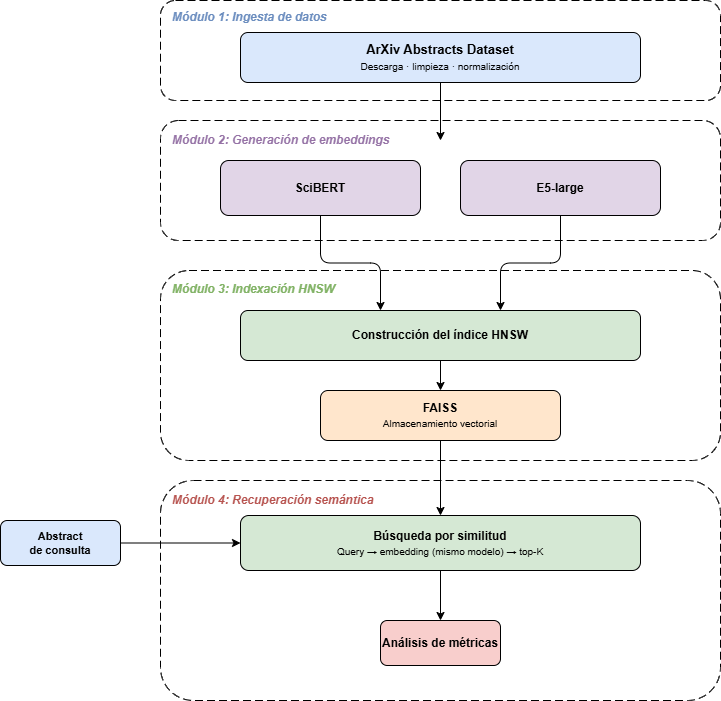
\includegraphics[width=0.85\textwidth]{Images/diagrama_bloques.png}
\caption{Diagrama de bloques del sistema: ingesta y muestreo del corpus,
vectorización mediante los modelos de embedding, indexación HNSW en FAISS y módulo
de evaluación de métricas.}
\label{fig:diagrama}
\end{figure}

% -------------------------------------------------------
\subsection{Visión general de la arquitectura}
% -------------------------------------------------------

La carga computacional se distribuye en función de sus requisitos de hardware. La
etapa de vectorización, intensiva en cómputo y dependiente de aceleración por GPU,
se ejecuta en Google Colab sobre una unidad NVIDIA T4. Las etapas de indexación y
evaluación se ejecutan localmente sobre CPU, entorno en el que la biblioteca FAISS
\cite{ref7} ofrece un rendimiento adecuado. La interfaz entre ambos entornos son
los vectores de embedding serializados: una vez generadas las representaciones, el
resto del procesamiento prescinde de la GPU.

Esta separación responde a un doble criterio. En primer lugar, reduce el costo
computacional al reservar el uso de GPU exclusivamente para la fase que lo requiere.
En segundo lugar, favorece la reproducibilidad del experimento: los procesos
estocásticos ---el muestreo estratificado y la selección del conjunto de
consultas--- quedan determinados por una semilla aleatoria compartida, de modo que
cada ejecución produce resultados equivalentes.

% -------------------------------------------------------
\subsection{Flujo de datos}
% -------------------------------------------------------

El procesamiento sigue una secuencia de etapas claramente delimitadas:

\begin{enumerate}
    \item \textbf{Ingesta y muestreo.} Se descarga el conjunto
    \textit{arxiv-abstracts-2021} \cite{ref17} y se aplica el muestreo estratificado
    por categoría hasta obtener los 50\,000 abstracts, de los cuales se reservan
    1\,000 como conjunto de consultas.
    \item \textbf{Vectorización.} Cada abstract se transforma en un vector denso
    mediante los modelos SciBERT \cite{ref18} y E5-large \cite{ref19}.
    \item \textbf{Cálculo del \textit{ground truth}.} Para cada par (modelo,
    métrica) se determinan los vecinos exactos de cada consulta mediante búsqueda por
    fuerza bruta.
    \item \textbf{Indexación y consulta.} Se construyen los 36 índices HNSW y se
    resuelven sobre cada uno las 1\,000 consultas.
    \item \textbf{Evaluación y exportación.} Se calculan Recall@K, MRR y latencia, y
    los resultados se consolidan en tablas.
\end{enumerate}

% -------------------------------------------------------
\subsection{Componentes y desarrollo}
% -------------------------------------------------------

El \textit{pipeline} se estructura en módulos de responsabilidad única, coordinados
por un archivo de configuración central que concentra las rutas, los hiperparámetros
y la semilla aleatoria. La ingesta del corpus se realiza con la biblioteca
\texttt{datasets}, mientras que la vectorización emplea \texttt{sentence-transformers}.
Dado que SciBERT es un modelo de tipo BERT que no incorpora una capa de agregación
propia, se añade una operación de \textit{pooling} de media para obtener un único
vector por documento \cite{ref3}; el modelo E5-large, por su parte, requiere los
prefijos \texttt{query:} y \texttt{passage:} establecidos durante su preentrenamiento.

La indexación y la recuperación se sustentan íntegramente en FAISS. El
\textit{ground truth} se obtiene con índices exactos (\texttt{IndexFlatL2} para
distancia euclídea e \texttt{IndexFlatIP} para producto interno), en tanto que las
36 configuraciones se construyen con \texttt{IndexHNSWFlat}, fijando el parámetro
\textit{ef\_construction} antes de la inserción y \textit{ef\_search} antes de la
consulta. La similitud coseno se implementa normalizando los vectores y aplicando
producto interno, dado que FAISS no la provee de forma nativa. Finalmente, el módulo
de evaluación consolida las métricas en un archivo CSV y las exporta de manera
automática a tablas en formato LaTeX, lo que elimina la transcripción manual de los
resultados.

% -------------------------------------------------------
\section{Resultados}
% -------------------------------------------------------

% TODO: Presentar métricas Recall@K, MRR y latencia obtenidas

\begin{table}[h]
\caption{Recall@K, MRR y latencia según modelo de embedding y métrica de similitud
sobre FAISS-HNSW (mejor configuración de $M$ y \textit{ef\_construction}).}
\label{tab:resultados}
\centering
\begin{tabular}{|l|l|c|c|c|c|c|}
\hline
\textbf{Modelo} & \textbf{Métrica} & \textbf{R@1} & \textbf{R@5} & \textbf{R@10}
& \textbf{MRR} & \textbf{Lat. (ms)} \\
\hline
SciBERT   & Coseno & -- & -- & -- & -- & -- \\
SciBERT   & L2     & -- & -- & -- & -- & -- \\
E5-large  & Coseno & -- & -- & -- & -- & -- \\
E5-large  & L2     & -- & -- & -- & -- & -- \\
\hline
\end{tabular}
\end{table}

% -------------------------------------------------------
\section{Conclusiones}
% -------------------------------------------------------

% TODO: Completar con conclusiones finales tras ejecutar los experimentos.

% -------------------------------------------------------
\section{Discusión}
% -------------------------------------------------------

% TODO: Análisis crítico de resultados, comparación con trabajos relacionados y
% líneas de trabajo futuro.

% -------------------------------------------------------
% Referencias — ordenadas por orden de primera aparición en el texto
% -------------------------------------------------------
\begin{thebibliography}{19}

\bibitem{ref1}
arXiv, ``arXiv Submission Statistics,'' Cornell University.\\
\url{https://arxiv.org/stats/monthly_submissions}, último acceso mayo 2026.

\bibitem{ref2}
U.S. National Library of Medicine, ``MEDLINE/PubMed Production Statistics.''\\
\url{https://www.nlm.nih.gov/bsd/medline_pubmed_production_stats.html},
último acceso mayo 2026.

\bibitem{ref3}
N. Reimers and I. Gurevych, ``Sentence-BERT: Sentence Embeddings Using Siamese
BERT-Networks,'' in \textit{Proc. 2019 Conf. Empirical Methods in Natural Language
Processing (EMNLP-IJCNLP)}, 2019, pp. 3982--3992.\\
\url{https://doi.org/10.18653/v1/D19-1410}

\bibitem{ref4}
S. Mathur and A. Chhabra, ``Vector Search Algorithms: A Brief Survey,'' in
\textit{Proc. Int. Conf. on Emerging Technologies}, IEEE, 2024.

\bibitem{ref5}
Y. A. Malkov and D. A. Yashunin, ``Efficient and Robust Approximate Nearest
Neighbor Search Using Hierarchical Navigable Small World Graphs,'' \textit{IEEE
Trans. Pattern Anal. Mach. Intell.}, vol. 42, no. 4, pp. 824--836, 2020.\\
\url{https://doi.org/10.1109/TPAMI.2018.2889473}

\bibitem{ref6}
D. J. Watts and S. H. Strogatz, ``Collective Dynamics of `Small-World' Networks,''
\textit{Nature}, vol. 393, no. 6684, pp. 440--442, 1998.\\
\url{https://doi.org/10.1038/30918}

\bibitem{ref7}
J. Johnson, M. Douze, and H. J\'egou, ``Billion-Scale Similarity Search with
GPUs,'' \textit{IEEE Trans. Big Data}, vol. 7, no. 3, pp. 535--547, 2021.\\
\url{https://doi.org/10.1109/TBDATA.2019.2921572}

\bibitem{ref8}
J. Wang \textit{et al.}, ``Milvus: A Purpose-Built Vector Data Management System,''
in \textit{Proc. ACM Int. Conf. Management of Data (SIGMOD)}, 2021,
pp. 2614--2627.\\
\url{https://doi.org/10.1145/3448016.3457550}

\bibitem{ref9}
F. Zhao, D. Liu, and Y. Wang, ``Hierarchical HNSW Index Construction Method Based
on Maximum Distance Constraint,'' in \textit{Proc. 5th Int. Conf. Digital Society
and Intelligent Systems (DSInS)}, IEEE, 2025.

\bibitem{ref10}
P. Lewis \textit{et al.}, ``Retrieval-Augmented Generation for Knowledge-Intensive
NLP Tasks,'' in \textit{Advances in Neural Information Processing Systems
(NeurIPS)}, vol. 33, 2020, pp. 9459--9474.\\
\url{https://doi.org/10.48550/arXiv.2005.11401}

\bibitem{ref11}
H. Elkiran and J. Rasheed, ``Systematic Evaluation of Similarity Metrics for
Retrieval, Reranking, and Completion in Retrieval Augmented Generation Systems,''
in \textit{Proc. IEEE Int. Conf. Emerging Trends in Engineering and Computing
(ETE-COM)}, IEEE, 2025.

\bibitem{ref12}
P. Rajpurkar, J. Zhang, K. Lopyrev, and P. Liang, ``SQuAD: 100,000+ Questions for
Machine Comprehension of Text,'' in \textit{Proc. 2016 Conf. Empirical Methods in
Natural Language Processing (EMNLP)}, 2016, pp. 2383--2392.\\
\url{https://doi.org/10.48550/arXiv.1606.05250}

\bibitem{ref13}
M. Iwasaki and D. Miyazaki, ``Optimization of Indexing Based on k-Nearest Neighbor
Graph for Proximity Search in High-Dimensional Data,'' arXiv preprint
arXiv:1810.07355, 2018.\\
\url{https://doi.org/10.48550/arXiv.1810.07355}

\bibitem{ref14}
X. Zhao, Y. Tian, K. Huang, B. Zheng, and X. Zhou, ``Towards Efficient Index
Construction and Approximate Nearest Neighbor Search in High-Dimensional Spaces,''
\textit{Proc. VLDB Endowment}, vol. 16, no. 8, pp. 1979--1991, 2023.\\
\url{https://doi.org/10.14778/3594512.3594527}

\bibitem{ref15}
H. J\'egou, M. Douze, and C. Schmid, ``Product Quantization for Nearest Neighbor
Search,'' \textit{IEEE Trans. Pattern Anal. Mach. Intell.}, vol. 33, no. 1,
pp. 117--128, 2011.\\
\url{https://doi.org/10.1109/TPAMI.2010.57}

\bibitem{ref16}
C. D. Manning, P. Raghavan, and H. Sch\"utze, \textit{Introduction to Information
Retrieval}. Cambridge University Press, 2008.

\bibitem{ref17}
C. B. Clement, M. Bierbaum, K. P. O'Keeffe, and A. A. Alemi, ``On the Use of ArXiv
as a Dataset,'' arXiv preprint arXiv:1905.00075, 2019.\\
\url{https://doi.org/10.48550/arXiv.1905.00075}

\bibitem{ref18}
I. Beltagy, K. Lo, and A. Cohan, ``SciBERT: A Pretrained Language Model for
Scientific Text,'' in \textit{Proc. 2019 Conf. Empirical Methods in Natural
Language Processing (EMNLP-IJCNLP)}, 2019, pp. 3615--3620.\\
\url{https://doi.org/10.18653/v1/D19-1371}

\bibitem{ref19}
L. Wang \textit{et al.}, ``Text Embeddings by Weakly-Supervised Contrastive
Pre-training,'' arXiv preprint arXiv:2212.03533, 2022.\\
\url{https://doi.org/10.48550/arXiv.2212.03533}

\end{thebibliography}

\end{document}
